\documentclass[table,xcdraw]{beamer}
\usetheme{Madrid}

\usepackage[utf8]{inputenc}
\usepackage{default}
\usepackage[T1]{fontenc}
\usepackage{wrapfig}
\usepackage[export]{adjustbox}
\usepackage{wrapfig}
\usepackage{verbatim}

\begin{document}

\title[MaldOS] % (optional, only for long titles)
{{\huge\textsc{MaldOS}:} \\
a Moderately Abstracted Layer for Developing Operating Systems}
\author[Mattia Maldini] % (optional, for multiple authors)
{Mattia Maldini\\[3mm]Relatore: Renzo Davoli\\[3mm]}

\institute[Università di Bologna] % (optional)
{
  Università di Bologna
}
\date[Laurea 2019] % (optional)
{Sessione di laurea 14 marzo 2019}
\subject{Informatica}

\frame{\titlepage}

\begin{frame}
    Structuring an Operating Systems course can be a thorny task. \\
    \bigskip
    Topics like
    scheduling, parallel programming, virtual memory and context switching are 
    hard to grasp via a purely abstract approach, and developing a concrete 
    example is inherently non trivial.\\
    \bigskip
    A previous solution to this issue was the $\mu$MPS family of emulators; this
    work proposes a slight shift in the form of an abstraction layer allowing for
    easier development on real hardware.
    \begin{comment}
        I sistemi operativi sono un argomento particolarmente spinoso nel contesto
        dell'insegnamento. I concetti che vengono coperti possono essere facilmente
        compresi a un livello superficiale e intuitivo, ma sono difficili da 
        interiorizzare senza un approccio pratico; approccio pratico che, considerata
        l'inerente complessita' dell'argomento, e' a sua volta complesso da
        applicare.
        Una soluzione seguita nel corso degli anni dal professor Davoli si appoggia
        a uMPS e simili, una famiglia di emulatori ad hoc per architettura MIPS 
        (e ARM).
        MaldOS e' una variazione sul tema; e' un acronimo per Moderately
        Abstracted Layer for Developing Operating Systems, ovvero un layer
        che renda piu' semplice (ma non troppo) l'approccio all'hardware di
        una architettura reale.
    \end{comment}
\end{frame}

\begin{frame}
    \frametitle{Tradeoffs}
    $\mu$MPS2 allows students to work in a simplified environment while still being
    faithful to the real MIPS architecture, providing an interesting experience.
    However
    \begin{itemize}
        \item it is still abstract work, as the resulting OS will never run on a real device
        \item $\mu$MPS is an ad-hoc emulator
        \item Its debugging facilities lack step-by-step execution of C code
        \item MIPS is a dated architecture
    \end{itemize}
    \begin{comment}
        uMPS riproduce fedelmente un'architettura reale, offrendo quindi un
        esempio didatticamente interessante, rimuovendo i dettagli che non
        sono interessanti per lo studio dei sistemi operativi. Per esempio, 
        l'interazione con le periferiche tramite registri e' considerata parte
        integrante dello sviluppo di un sistema operativo; l'elevata complessita'
        dei protocolli di controllo di suddette periferiche e' invece un ostacolo
        all'apprendimento.
        uMPS cerca quindi di trovare un equilibrio tra un lavoro concreto (e quindi interessante)
        e un ambiente virtuale piu' accessibile per gli studenti. Riesce in questo
        obbiettivo, ma con alcuni caveat:
        Pur appoggiandosi a un'architettura reale, la macchina uMPS e' comunque
        astratta e inesistente; il lavoro sviluppato non trova quindi corrispondenze
        al di fuori dell'emulatore.
        Per quanto sia un tool ben sviluppato si tratta di un progetto accademico
        di nicchia; gli studenti imparano ad usarlo e lo dimenticano dopo l'esame.
        Offre delle visualizzazioni di debug specifiche e sofisticate, ma ha il
        grande difetto di non permettere l'esecuzione step-by-step del codice C.
        Infine, MIPS e' un'architettura ormai datata, e per gli studenti puo'
        essere piu' interessante studiare ambienti piu' moderni e diffusi, come ARM.
    \end{comment}
\end{frame}

\begin{frame}
    \frametitle{Tradeoffs}
    \textbf{MaldOS} is an abstraction layer devised to reproduce an $\mu$MPS-like simplified
    environment on a real device and architecture, the Raspberry Pi 3 and ARMv8.
    \begin{itemize}
        \item it is an extremely practical example, and the result can be run on a real machine
        \item it relies on general purpose software (namely, Qemu and GDB)
        \item its debugging facilities are less specific but more powerfull (full GDB support)
        \item ARM is a more modern and widespread environment
    \end{itemize}
    \begin{comment}

    \end{comment}
\end{frame}

\begin{frame}
    \frametitle{Bare Metal}
    The problem with a real architecture is the intrinsic complexity of hardware
    management. The abstraction layer softens the approach by partially taking care 
    of initialization and configuration procedures.
    \begin{figure}[b]
    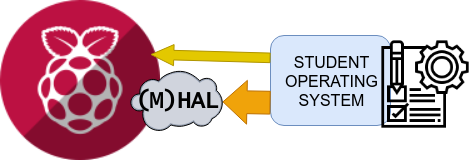
\includegraphics[scale=0.7]{raspberrypi.png}
    \end{figure}
\end{frame}

\begin{frame}
    \frametitle{Initialization}
    \begin{itemize}
        \item Move to the correct level of execution
        \item Prepare memory structure (stack pointers and such)
        \item Boot all four kernels and park them
        \item Prepare the C environment (zero bss section)
        \item Configure and initialize all real devices (UART, screen, SD)
    \end{itemize}
\end{frame}

\begin{frame}
    \frametitle{Interrupt Management}
    \makebox[\linewidth]{
        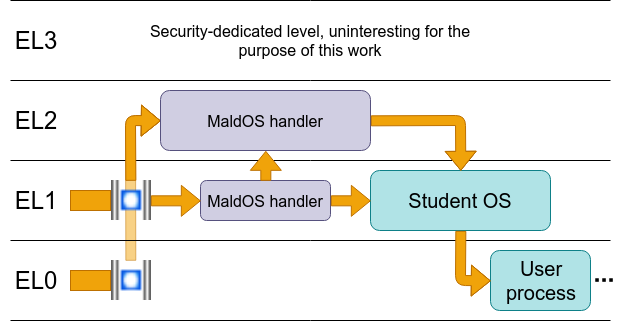
\includegraphics[scale=0.58]{execution_levels.png}
    }
\end{frame}

\begin{frame}
    \frametitle{Emulated Devices}
    \textbf{MaldOS} creates $\mu$MPS-style emulated devices with an ideal interface.
    Thanks to the mailbox interface the integration is seamless.

    \bigskip
    \begin{minipage}{0.49\textwidth}
        \begin{table}[]
            \begin{tabular}{|c|}
            \hline
            \rowcolor[HTML]{9B9B9B} 
            Virtual Disk device registers \\ \hline
            status register       \\ \hline
            command register      \\ \hline
            data 0 register       \\ \hline
            data 1 register       \\ \hline
            mailbox register      \\ \hline
            \end{tabular}
        \end{table}
    \end{minipage}
    \begin{minipage}{0.49\textwidth}
        \begin{table}[]
            \begin{tabular}{c}
            \hline
            \rowcolor[HTML]{9B9B9B} 
            \multicolumn{1}{|c|}{\cellcolor[HTML]{9B9B9B}EMMC device registers} \\ \hline
            \multicolumn{1}{|c|}{second argument register}                      \\ \hline
            \multicolumn{1}{|c|}{block size count register}                     \\ \hline
            \multicolumn{1}{|c|}{first argument register}                       \\ \hline
            \multicolumn{1}{|c|}{command register}                              \\ \hline
            \multicolumn{1}{|c|}{response registers (4)}                        \\ \hline
            \multicolumn{1}{|c|}{status register}                               \\ \hline
            \multicolumn{1}{|c|}{control register (2 of 3)}                     \\ \hline
            \multicolumn{1}{|c|}{interrupt register}                            \\ \hline
            \multicolumn{1}{|c|}{interrupt mask register}                       \\ \hline
            \multicolumn{1}{r}{... 11 more}                                    
            \end{tabular}
            \end{table}
    \end{minipage}

\end{frame}

\begin{frame}
    \frametitle{Virtual Memory}
    \vspace{-2cm}
    \begin{wrapfigure}{r}{0.65\textwidth}
        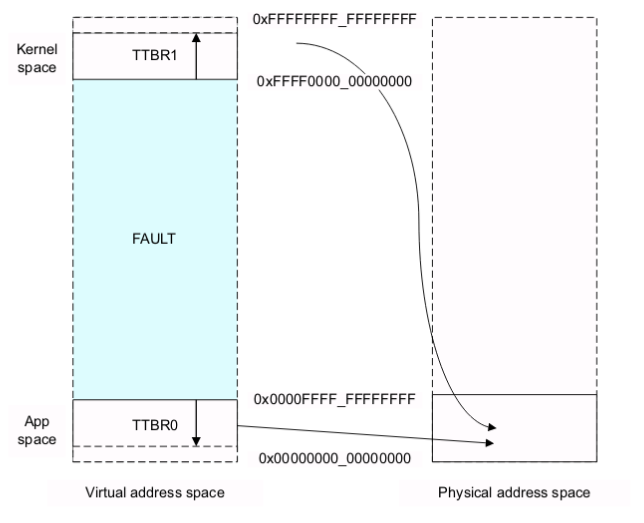
\includegraphics[scale=0.35]{ttbr.png}
    \end{wrapfigure}
    The ARMv8 MMU is remarkably flexible, so the virtual memory configuration is left
    mostly untouched.
    Students are assisted by changing page tables every time the kernel context
    switched in.
\end{frame}

\begin{frame}[plain]
    \frametitle{Qemu and Debugging}
    \makebox[\linewidth]{
        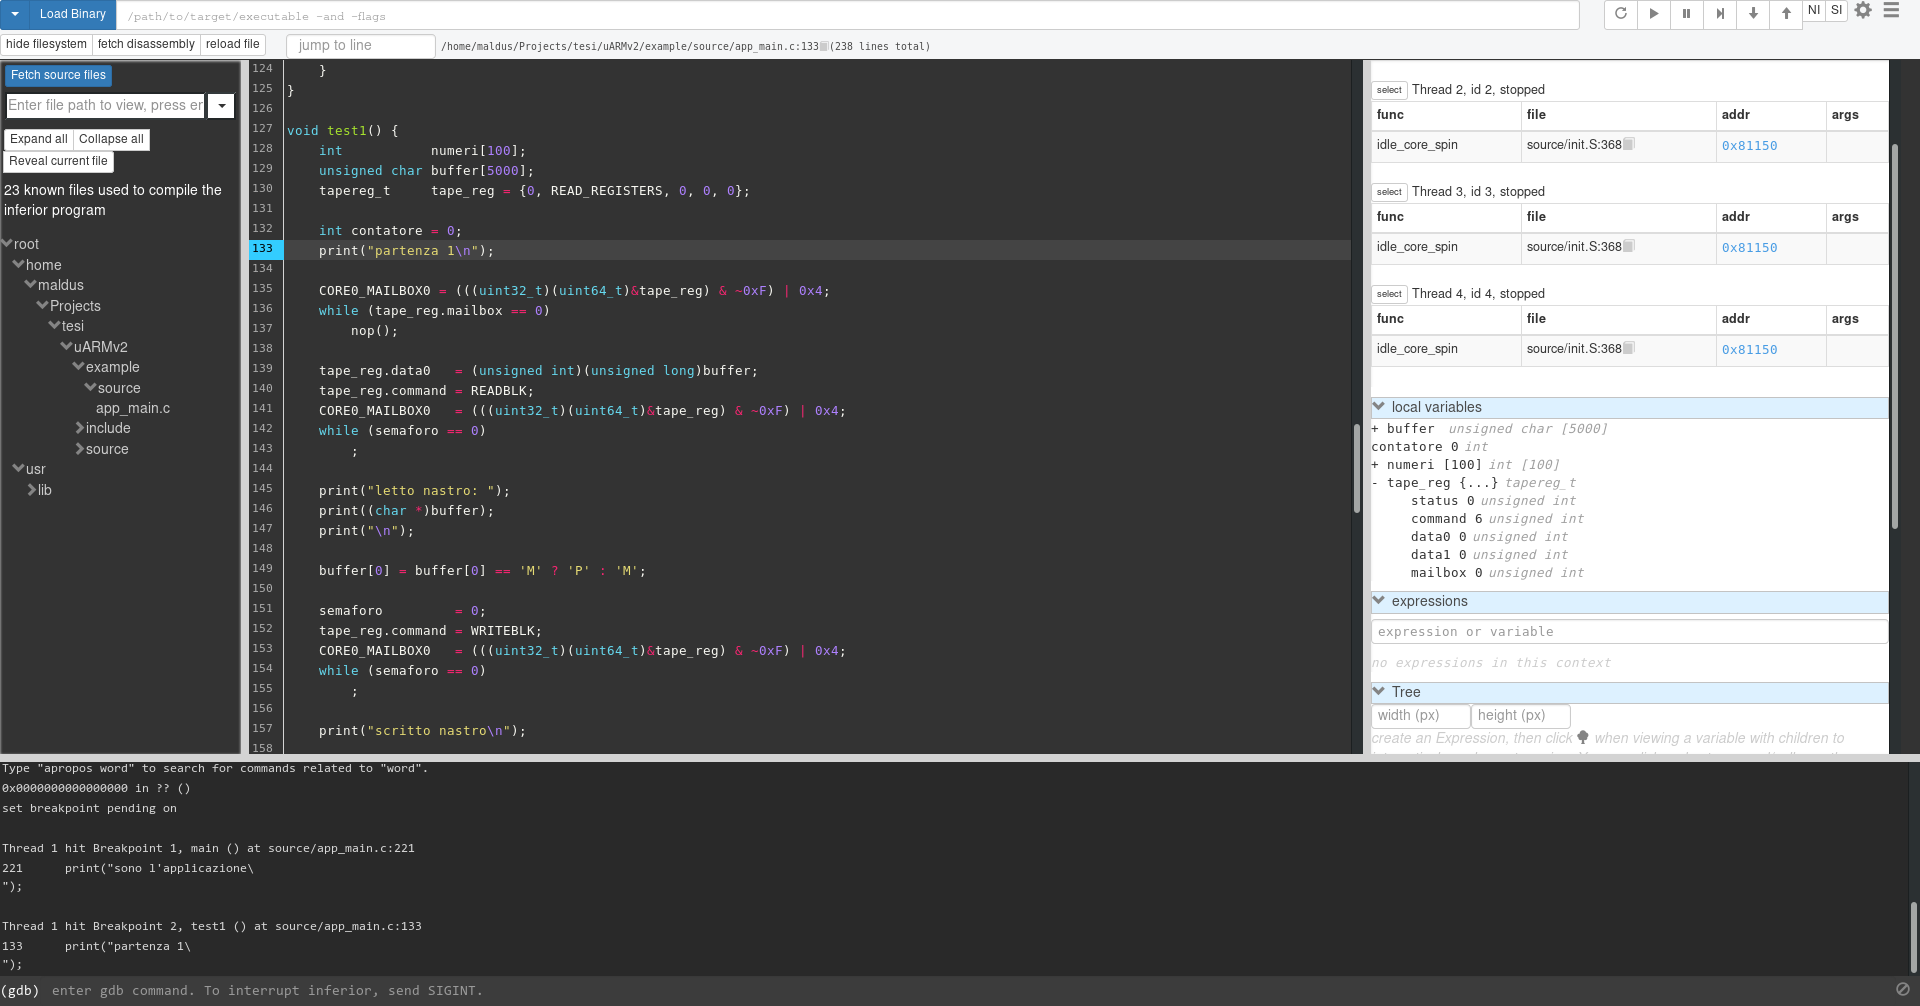
\includegraphics[width=12.5cm,height=8cm]{gdbgui.png}
    }
\end{frame}

\end{document}